\documentclass[10pt]{beamer}
\usefonttheme{professionalfonts} % using non standard fonts for beamer
\usefonttheme{serif} % default family is serif
\usepackage{amsmath}
\usepackage[normalem]{ulem}
\usepackage{ulem}
\usepackage{array}
\usepackage{mathtools}
%\documentclass[12pt]{beamerthemeSam.sty}
\usepackage{epsf}
%\usepackage{pstricks}
%\usepackage[orientation=portrait,size=A4]{beamerposter}
\geometry{paperwidth=160mm,paperheight=120mm}
%DT favorite definitions
\def\LL{\left\langle}	% left angle bracket
\def\RR{\right\rangle}	% right angle bracket
\def\LP{\left(}		% left parenthesis
\def\RP{\right)}	% right parenthesis
\def\LB{\left\{}	% left curly bracket
\def\RB{\right\}}	% right curly bracket
\def\PAR#1#2{ {{\partial #1}\over{\partial #2}} }
\def\PARTWO#1#2{ {{\partial^2 #1}\over{\partial #2}^2} }
\def\PARTWOMIX#1#2#3{ {{\partial^2 #1}\over{\partial #2 \partial #3}} }

\def\rightpartial{{\overrightarrow\partial}}
\def\leftpartial{{\overleftarrow\partial}}
\def\diffpartial{\buildrel\leftrightarrow\over\partial}

\def\BI{\begin{itemize}}
\def\EI{\end{itemize}}
\def\BE{\begin{displaymath}}
\def\EE{\end{displaymath}}
\def\BEA{\begin{eqnarray*}}
\def\EEA{\end{eqnarray*}}
\def\BNEA{\begin{eqnarray}}
\def\ENEA{\end{eqnarray}}
\def\EL{\nonumber\\}
\def\BS{\bigskip}
\def\BC{\begin{center}}
\def\EC{\end{center}}
\def\BCC{\begin{columns}}
\def\ECC{\end{columns}}
\def\HC{\column{0.5\textwidth}}

\newcommand{\etal}{{\it et al.}}
\newcommand{\gbeta}{6/g^2}
\newcommand{\la}[1]{\label{#1}}
\newcommand{\ie}{{\em i.e.\ }}
\newcommand{\eg}{{\em e.\,g.\ }}
\newcommand{\cf}{cf.\ }
\newcommand{\etc}{etc.\ }
\newcommand{\atantwo}{{\rm atan2}}
\newcommand{\Tr}{{\rm Tr}}
\newcommand{\dt}{\Delta t}
\newcommand{\op}{{\cal O}}
\newcommand{\msbar}{{\overline{\rm MS}}}
\def\chpt{\raise0.4ex\hbox{$\chi$}PT}
\def\schpt{S\raise0.4ex\hbox{$\chi$}PT}
\def\MeV{{\rm Me\!V}}
\def\GeV{{\rm Ge\!V}}

%AB: my color definitions
%\definecolor{mygarnet}{rgb}{0.445,0.184,0.215}
%\definecolor{mygold}{rgb}{0.848,0.848,0.098}
%\definecolor{myg2g}{rgb}{0.647,0.316,0.157}
\definecolor{abtitlecolor}{rgb}{0.0,0.255,0.494}
\definecolor{absecondarycolor}{rgb}{0.0,0.416,0.804}
\definecolor{abprimarycolor}{rgb}{1.0,0.686,0.0}
\definecolor{Red}           {cmyk}{0,1,1,0}
\definecolor{Grey}           {cmyk}{.7,.7,.7,0}
\definecolor{Lg}           {cmyk}{.4,.4,.4,0}
\definecolor{Blue}          {cmyk}{1,1,0,0}
\definecolor{Green}         {cmyk}{1,0,1,0}
\definecolor{Brown}         {cmyk}{0,0.81,1,0.60}
\definecolor{Black}         {cmyk}{0,0,0,1}
\definecolor{A}{rgb}{0.8,0.0,0.0}
\definecolor{B}{rgb}{0.0,0.6,0.0}
\definecolor{C}{rgb}{0.6,0.6,0.0}
\definecolor{D}{rgb}{0.0,0.0,0.5}
\definecolor{E}{rgb}{0.4,0.4,0.4}


\usetheme{Madrid}


%AB: redefinition of beamer colors
%\setbeamercolor{palette tertiary}{fg=white,bg=mygarnet}
%\setbeamercolor{palette secondary}{fg=white,bg=myg2g}
%\setbeamercolor{palette primary}{fg=black,bg=mygold}
\setbeamercolor{title}{fg=abtitlecolor}
\setbeamercolor{frametitle}{fg=abtitlecolor}
\setbeamercolor{palette tertiary}{fg=white,bg=abtitlecolor}
\setbeamercolor{palette secondary}{fg=white,bg=absecondarycolor}
\setbeamercolor{palette primary}{fg=black,bg=abprimarycolor}
\setbeamercolor{structure}{fg=abtitlecolor}

\setbeamerfont{section in toc}{series=\bfseries}

%AB: remove navigation icons
\beamertemplatenavigationsymbolsempty
\title{
  \textbf {Introduction}\\
%\centerline{}
%\centering
%\vspace{-0.0in}
%\includegraphics[width=0.3\textwidth]{propvalues_0093.pdf}
%\vspace{-0.3in}\\
%\label{intrograph}
}

\author[W. Freeman] {Physics 211\\Syracuse University, Physics 211 Spring 2022\\Walter Freeman}

\date{\today}

\begin{document}

\frame{\titlepage}

\frame{\frametitle{\textbf{Welcome!}}

\Huge
\begin{center}
Physics 211 \\
Forces and Motion\\

\bigskip

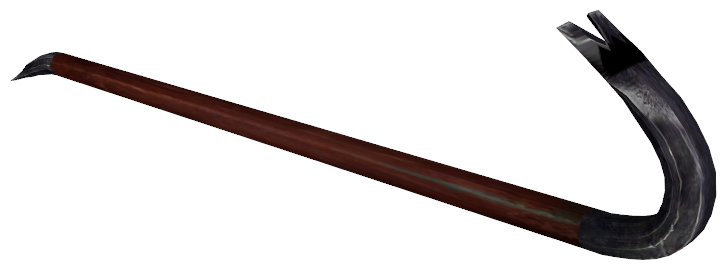
\includegraphics[width=0.3\textwidth]{crowbar.jpg}\\
\Large

\bigskip

Course webpage:

\Huge
http://walterfreeman.github.io/phy211/
\end{center}
}

\frame{
	
	\Large
	\BC
	
	Course Discord server: \url{https://discord.gg/bngYwjZRHk}
	
	(link also on the webpage)
	
	\BS\BS


\includegraphics[width=0.4\textwidth]{discord-qr.png}

\BS\BS


Come say hi; I and our teaching staff monitors this server and can provide assistance
pretty quickly most of the time.


\BS\BS

\EC

}

	
	

\frame{\frametitle{\textbf{Overview of today}}

\Large

\begin{itemize}
\item{Introduction to physics and mechanics}
\item{Course organization / syllabus}
\item{How to succeed in this course}
\item{{\color{Green}} Describing the physical world: the SI system}
\item{{\color{Red}} Mathematics in the context of physics}
\end{itemize}
}

\frame{\frametitle{\textbf{So what is this class?}}

\Large
\begin{center}
Physics: what are the fundamental laws of nature?

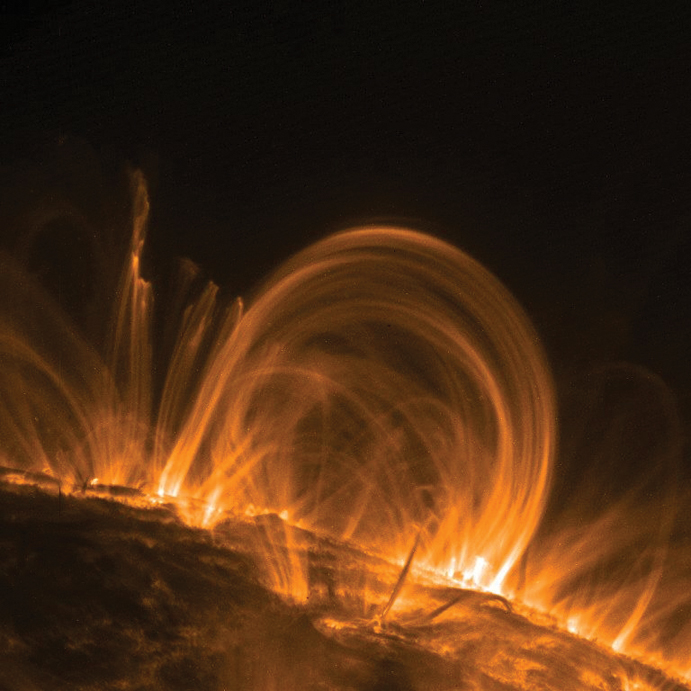
\includegraphics[width=0.27\textwidth]{sun.jpg}
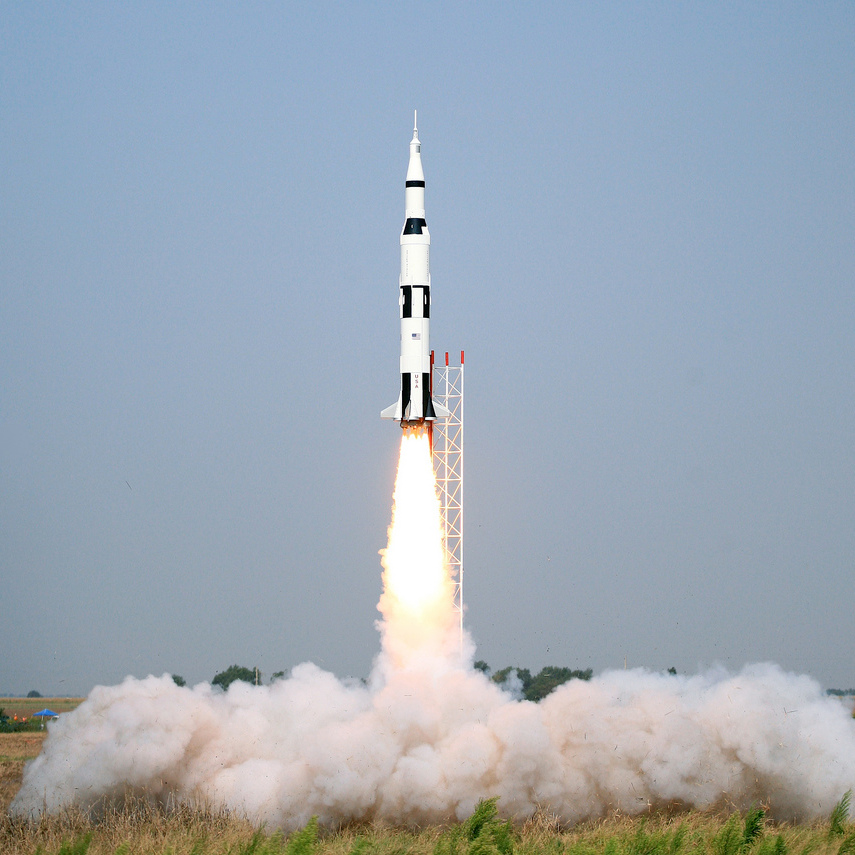
\includegraphics[width=0.27\textwidth]{rocket.jpg}
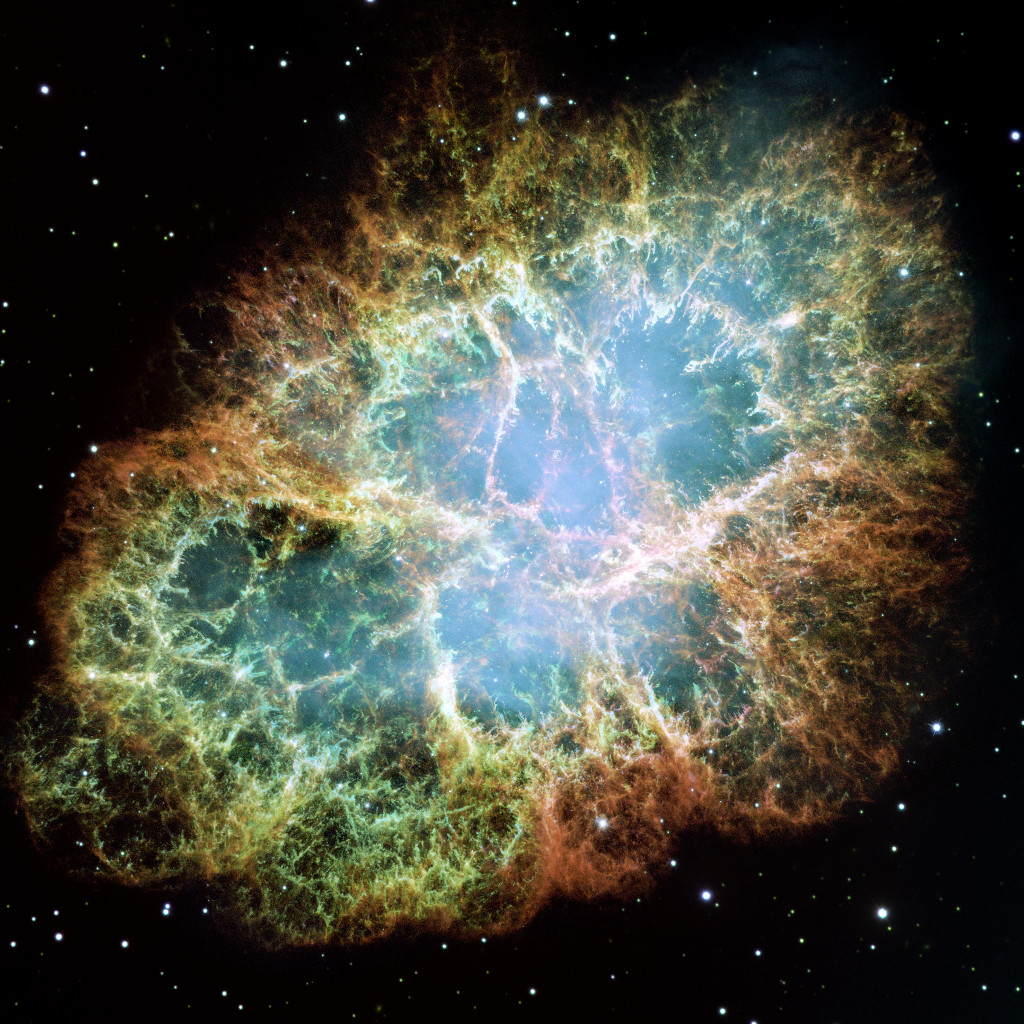
\includegraphics[width=0.27\textwidth]{crab-nebula.jpg}\\
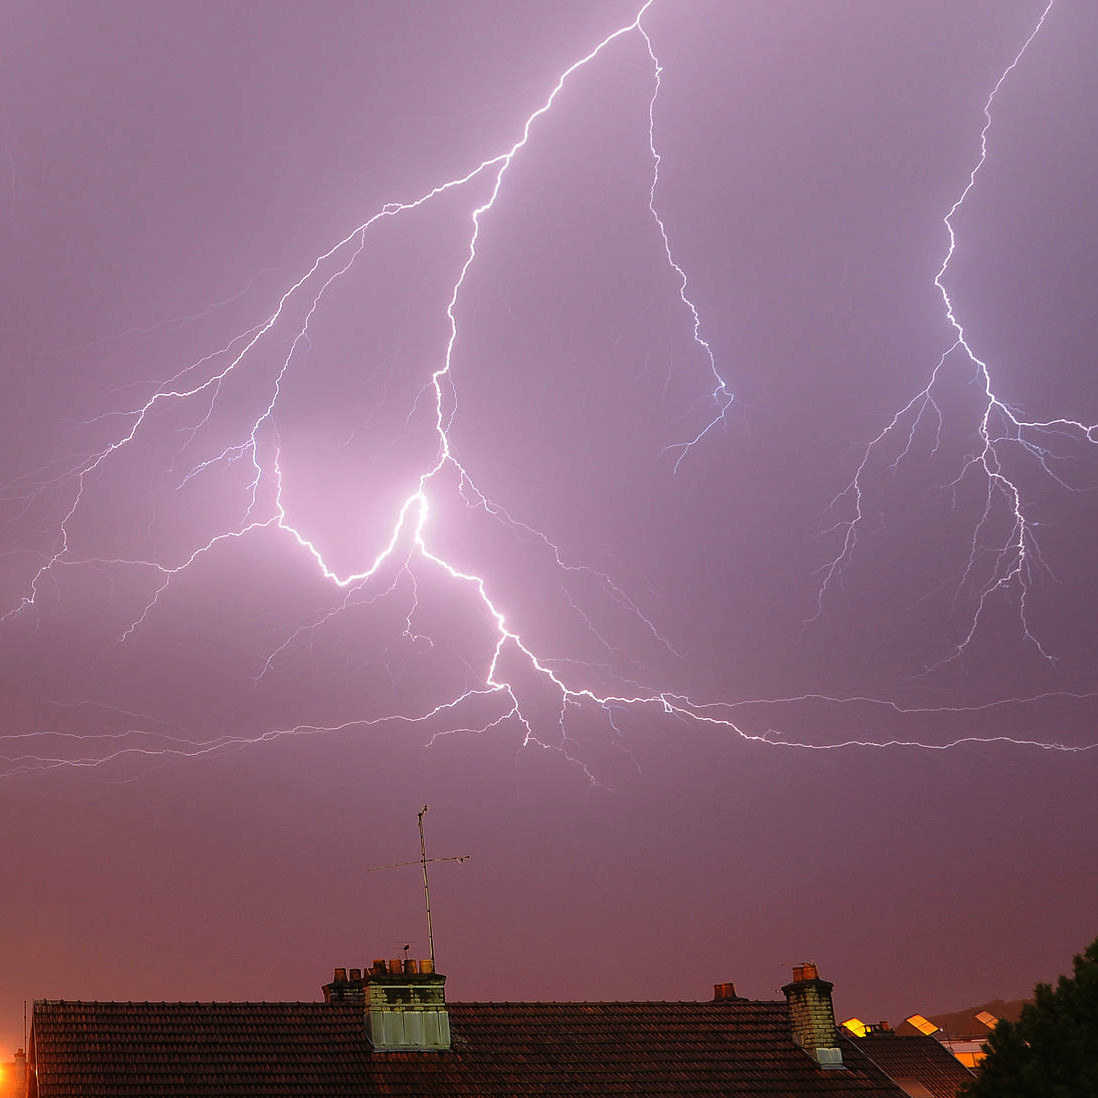
\includegraphics[width=0.27\textwidth]{lightning.jpg}
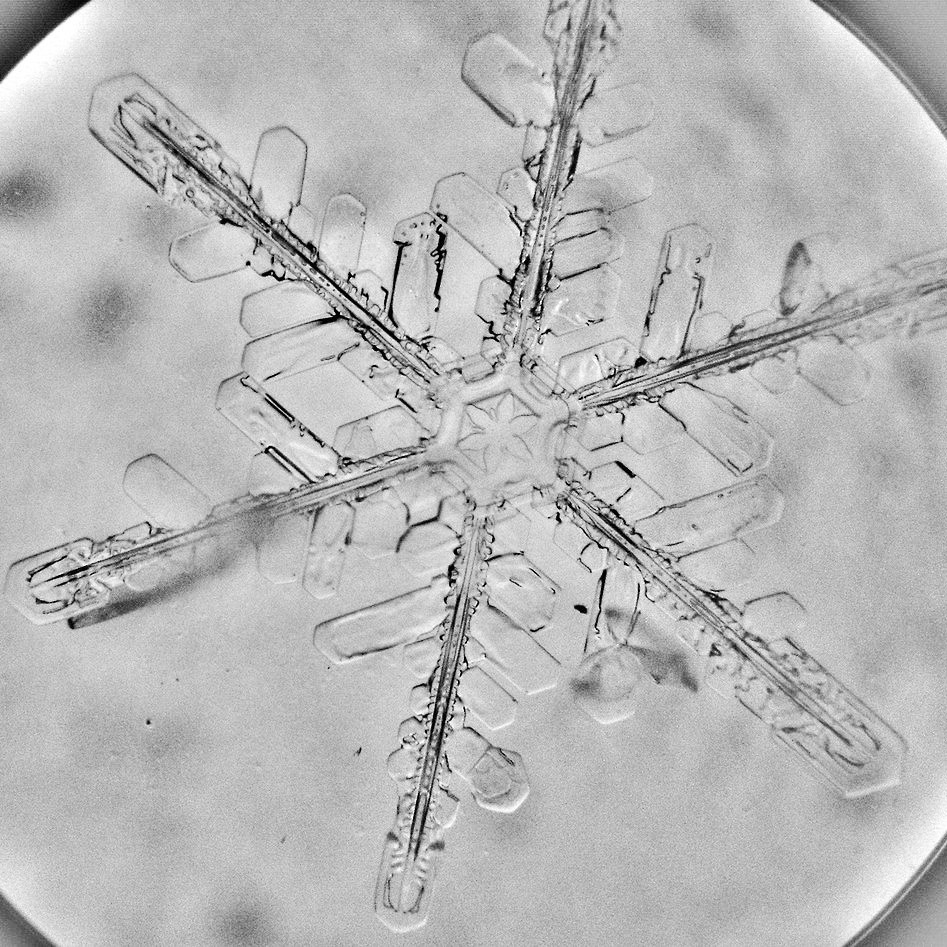
\includegraphics[width=0.27\textwidth]{snowflake.jpg}
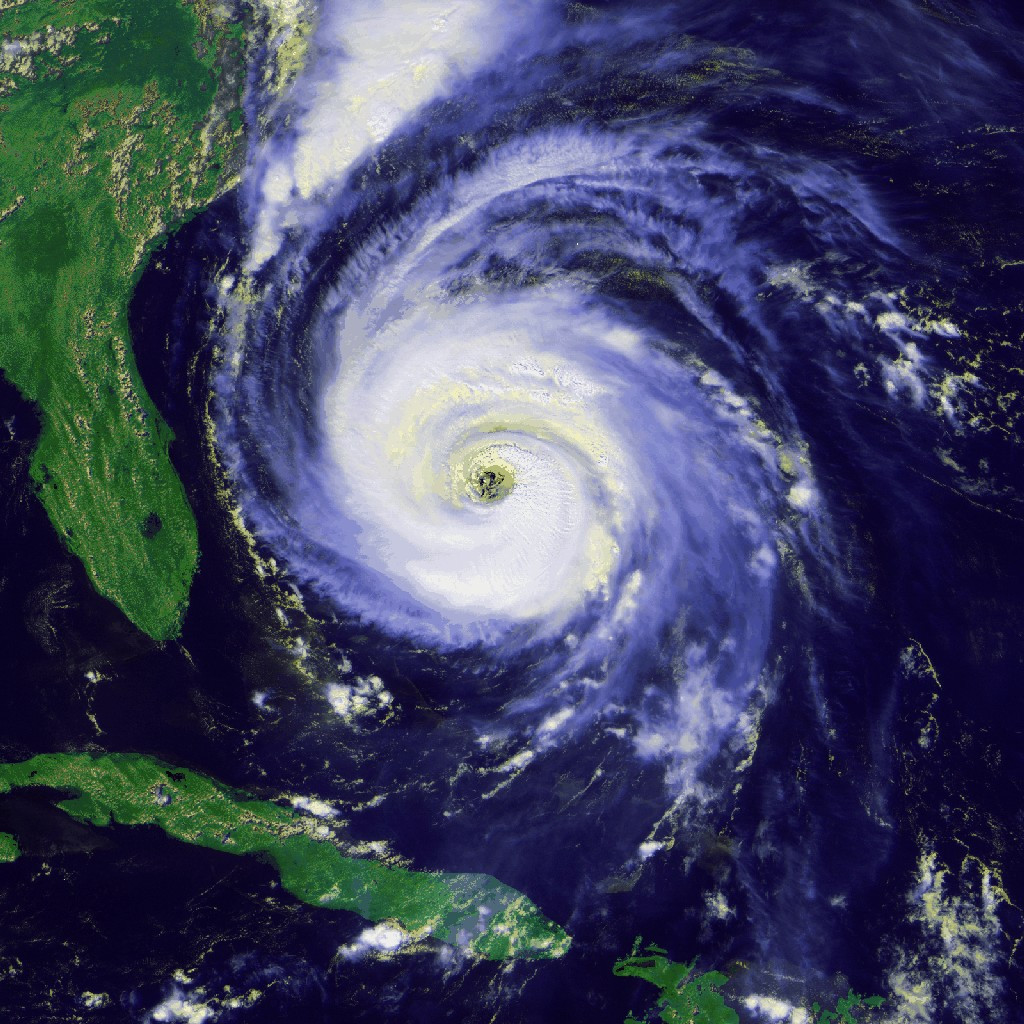
\includegraphics[width=0.27\textwidth]{hurricane.jpg}\\
These phenomena are all governed by the {\it same few principles}.
\end{center}
}

\frame{\frametitle{\textbf{Mechanics}}

\large The most fundamental question physics asks:

\bigskip

\Large \centerline{\color{Red}``Why do things move in the ways that they do?''}


\bigskip

\large

The answer is given by Isaac Newton's second law of motion:


\bigskip

\begin{center}
\Large {\color{Blue} ``Objects accelerate when pushed by forces; they accelerate in the direction of the force, proportional to the size of the force divided by their mass.''}
\end{center}
\normalsize


\bigskip
\large
That's it. We will spend much of our class talking about the meaning and consequences of this one statement.

\BS\pause

Let's see an example...


}


\frame{\frametitle{\textbf{The physicist's eye}}

\large

Physics is about {\color{Blue} understanding complicated things in terms of simple pieces}, like Newton's law.

\pause
\bigskip

The perspective of physics is one that looks at a situation and asks:

\begin{itemize}
\item{``What phenomena are involved in this thing?''}
\item{``How do they interact to determine its behavior?''}
\end{itemize}
\pause
\bigskip

In this class, you'll learn about some of those simple pieces, but that's not the important thing.

\bigskip

You'll also learn the skill of asking those two questions, and develop {\color{Blue}a physicist's perspective for solving problems}.

\bigskip

This will serve you well in whatever field you pursue, since the ability to quickly look at a problem and understand the crucial 
elements is universally helpful.

\bigskip

\pause

\color{Red}It turns out that people with physics training find good jobs all over industry, even in non-STEM fields, because of this skill!

}

\frame{\frametitle{\textbf{Why study physics?}}
	
	\begin{columns}
		\column{0.5\textwidth}
		
		
		
		``The {\bf \color{Red} far-reaching expertise} that physics students develop while receiving their degrees--through exposure to a broad set of skills and techniques--makes them {\bf \color{Red}exceptional problem solvers.} Moreover, their ability to {\bf \color{Red}approach problems from general principles} often means that physicists can {\bf \color{Red}apply their knowledge in novel contexts}, leading to innovative advances in technological development. Their intimate {\bf \color{Red}understanding of the laws of the universe}, along with the ability to harness the {\bf \color{Red}powerful machinery of mathematics to model and predict}, puts physics students in a unique position to tackle some of the world's biggest challenges.''
		
		
		
		\column{0.5\textwidth}
		``As a physicist, you have scientific, technical, and problem-solving skills that are valuable in a wide range of employment sectors. You have learned to {\bf \color{Green}approach problems from first principles} and can serve as a {\bf \color{Green}generalist when collaborating on interdisciplinary teams}. You understand how to set up and run experiments, analyze data, and create mathematical or computational models. {\bf \color{Blue}Most importantly, you have the confidence to advance beyond the edge of what is known... This habit of continued learning is a hallmark of a physicist, and greatly valued in all employment sectors.}''
		
		
		
	\end{columns}
	
	\begin{columns}
		\column{0.5\textwidth}
		\begin{flushright}
			--Crystal Bailey, American Physical Society, in the Careers 2020 report
		\end{flushright}
		\column{0.5\textwidth}
		\begin{flushright}
			--Kate Kirby, American Physical Society, in the Careers 2020 report
		\end{flushright}
	\end{columns}
	
}



\frame{\frametitle{\textbf{Course structure and syllabus review}}
\centerline{\Large{Four broad sections:}}
\bigskip
\Large
\begin{enumerate}
\item{Kinematics (understanding the right hand side of $\vec F=m \vec a$)}
\begin{itemize}
\item{How do we describe motion?}
\item{How do an object's position, velocity, and acceleration relate?}
%\item{{\color{Red}What about rotational motion?}}
\item{How do we deal with things in two or three dimensions?}
\end{itemize}
\pause
\item{Forces and motion (both sides of $\vec F=m \vec a$)}
\begin{itemize}
\item{What kinds of forces are there?}
%\item{{\color{Red}Torque: a rotational counterpart to force, with an equivalent to $\vec F = m \vec a$}}
\item{Understanding different physical situations using $\vec F = m \vec a$}
\item What kinds of forces are required to make things move in different ways?
\end{itemize}
\pause
\item{Conservation laws: when you want to do less math}
\begin{itemize}
\item{Energy: a way to simplify solving $\vec F = m \vec a$ when you don't care about time}
\item{Momentum: a way to simplify problems involving collisions and explosions}
\item Rotational energy and angular momentum: the equivalents for rotating things
\end{itemize}
\item Two more mechanics topics
\BI
\item Rotational motion in detail
\BI
\item How do forces cause things to rotate?
\item What does it mean for an object to {\it roll}?
\EI
\item What properties do waves and vibrations have?
\BI
\item What happens to waves when they are trapped?
\item What are the physics of music and musical instruments?
\item How does this relate to chemistry, biology, and engineering?
\EI

\EI


\end{enumerate}
}
%
%\frame{\frametitle{\textbf{The process of science}}
%	
%	\large
%	
%	In this class, we won't just be studying the things physics has discovered.
%	
%	\bigskip\bigskip
%	
%	We'll also be studying {\it what physics, and science more broadly, is.}
%	
%	\bigskip\bigskip\pause
%	
%	Science has been a uniquely powerful way to learn about our world.
%	
%	\bigskip
%	
%	It is, at its heart, a way to avoid fooling yourself.\pause
%	
%	\bigskip\bigskip
%	
%	But this can go wrong in two ways:
%	
%	\begin{itemize}
%		\color{Red}
%		\item If someone's not careful they might fool yourself or other people (innocent error)
%		\item If someone's not honest they can disguise phony conclusions as science and deliberately mislead other people (pseudoscience)
%	\end{itemize}
%	
%	\bigskip
%	
%	We'll study what science is, what it's not, and how you can protect yourself from \sout{bullshit} flawed scientific reasoning.
%
\frame{\frametitle{\textbf{Clickers}}
\Large
You all should have gotten a clicker from the bookstore.

\pause
\bigskip
\bigskip
\bigskip

... wait, you didn't?

\begin{columns}

\begin{column}{0.5\textwidth}
\end{column}
\pause
\begin{column}{0.5\textwidth}
...Maybe we have some extras...

\pause

\bigskip


\includegraphics[width=0.6\textwidth]{trollface.png}

\pause

\end{column}
\end{columns}
\bigskip
\bigskip

We're using an extremely high-tech, state-of-the-art clicker system in this class.
Make sure you get one, and bring it to class every day.
\pause
\begin{center}
	\small \it (This slide will be much less funny if we are out of them!)
\end{center}

}

\frame{\frametitle{\textbf{Syllabus review}}
\BI
\Large
\item Our philosophy
\item How grading works
\item The components of the course
\item Academic integrity 
\pause
\item Dealing with COVID
\EI
}

\frame{\frametitle{\textbf{Recitations}}
\BI
\normalsize
\item{Discussion sections led by TA's and coaches}
\item{Homework is submitted and returned in recitation}
\item{{\bf Crucial} for your success in this class} -- more important than anything else
\pause
\item {\color{Green}Recitation is not ``support'' for the class meeting}
\pause
\item {\color{Red}...the class meeting really exists to get you ready for recitation!}
\pause
\EI
\BS
\Large
In recitation:
\BI
\normalsize
\item You will work in groups of three on exercises
\item We'll have lots of teaching staff around to help you
\item{You will work together for a whole unit and then have a ``group exam''}
\EI

\BS

\Large Remember:
\BI
\normalsize
\item{Physics is not about how much you know -- it's about {\bf what you can do}}
\item{This class isn't about amassing facts; it's about solving problems}
\item{This takes practice, and the recitations (and the homework) are where you get it}
\item{We have a large and talented group of instructors this year; make use of them!}
\EI
}

\frame{\frametitle{\textbf{The course webpage}}
\large
\BI
\item{All notes, etc., will be posted on the course website}
\item{I will also post course announcements there}
\item{The syllabus is posted there, as is a FAQ}
\item{You really should read the section on the course philosophy in the syllabus}
\EI
}

\frame{\frametitle{\textbf{How to do well in this class (important!)}}
\Large
\centerline{This class isn't about learning facts or memorizing equations!}
\pause
\bigskip
\large
In this class, we hope you will:
\BI
\item{... learn to look at moving things around you in a new, rigorous way}
\pause
\item{... learn to solve problems by taking them apart, understanding the parts, and putting them back together again}
\pause
\item{... learn to translate between and combine verbal, visual, and mathematical descriptions of things, while still being precise}
\pause
\EI

\BS\BS

\centerline{These things are skills, and they all require practice}
\centerline{... but they also require you to ask questions and ask for guidance!}
}

\frame{\frametitle{\textbf{How to do well in this class: ask for guidance!}}
\Large
\begin{center}
Some students might come to class, write down everything,
go home and review, and then spend hours alone working on the homework. They're 
diligent, good, hardworking students, right?
\end{center}
\pause

\bigskip

\centerline{... but this is not the best way to learn skills! Instead, we hope you will:}
\medskip

\large
\BI
\item Ask questions in class (we will often set aside time for homework questions)
\item{Interrupt me in class and ask questions about the presentation}
\item {\color{Red}Talk to me, your peers, and the teaching staff on the Discord server}
\pause
\item Ask me questions over email
\item{Come work with us and with your peers in our help sessions}
\item{Do your homework in the Physics Clinic when you can}
\EI
}

\frame{\frametitle{\textbf{Metaphors: sports and music}}
\large

Learning physics is like learning to play a musical instrument.

\bigskip

The hard part isn't learning the notes -- it's being able to play them, and tell a story with them.

\bigskip

How does studying the piano work?

\begin{itemize}
\item{Your teacher shows you a few techniques, and gives you a piece to learn to play}
\item{You take it home, practice it, and get stuck on difficult parts}
\item{You ask your teacher for advice; they guide you}
\item{You practice some more}
\item{You repeat the previous steps until you've mastered the technique and the music}
\item Over time, you become fluent in music as a new language
\end{itemize}

\bigskip

Physics is like this. We don't expect you to master everything immediately; physics takes practice, and it's
okay to get stuck and ask questions. In fact, it's what we expect!
}

\frame{\frametitle{\textbf{The Physics Clinic}}
\large
The Clinic is in room 112; it's a large room with tables, boards, 
and (usually) a graduate teaching assistant. Often the professors and coaches are there, too.

\bigskip

You can go there whenever the building is open to work in groups on your homework, and
ask each other and the GTA for help.

\bigskip

I also hold help hours there. They'll fluctuate based on when homework is due. 

\BS

{\color{Red}This week I'll be in the Physics Clinic Tuesday 2-4pm and Friday 12-2pm.}

\bigskip

This is an excellent resource for you to use; why do your homework alone when you can work
with your peers and instructors? 
}

\frame{\frametitle{\textbf{The course Discord server}}

Last year the course Discord server was home to a nearly 24-hour 
conversation, with students getting help from me, the GTA's and coaches, and each other.

\BS

It also became a social space, and many of our students found that
their classmates are nifty folks.


\BC
\includegraphics[width=0.6\textwidth]{celebration.jpg}
\EC


}
\frame{\frametitle{\textbf{Office hours}}

\Large
You're also always free to drop by my office: Physics 215 (the one with the birds on the door)


\bigskip

I might not be there, and I might have other urgent stuff to do, but helping students learn is a very high priority, so 
if I'm around, likely I can drop whatever I'm doing and help you with physics.

}

\frame{\frametitle{\textbf{Dimensions}}
\large
Things in nature aren't just described by numbers; they have an associated {\it dimension},
and we measure them using a {\it system of units}.

\BS

We have three different kinds of dimension:

\Large

\BI
\item {\bf Length}: usually measured in {\bf meters}; also inches, miles, light-years...
\item {\bf Mass}: usually measured in {\bf kilograms}; also grams, tonnes...
\item {\bf Time}: usually measured in {\bf seconds}; also hours, days...
\EI

\pause

\BS

For the Americans: the pound measures {\it force}, not mass. The word 
``weight'' means ``force due to gravity''; an object with a mass of
one kilogram weighs 2.2 pounds on Earth.
}

\frame{\frametitle{\textbf{Math, physics-style, I: working with dimensions}}
\Large

\BC ``It is two hours from Syracuse to Adirondack State Park'' \EC

\BS

Does this statement make sense?

\Huge

\color{A}A: Yes\\
\color{B}B: No\\
\pause
\color{C}C: Only if I tell you something else, too\\

\pause

\Large
\color{Black}
\BS
\BC
I've got to also tell you the car's velocity!
\EC
}

\frame{\frametitle{\textbf{Math, physics-style, I: working with dimensions}}

\Large

\BC

``The distance from Syracuse to the Adirondacks is two hours''


$$\color{Red} {\rm Distance} \color{Black} = \color{Green} {\rm Time}$$


{\bf This statement makes no sense!}

\BS\BS\BS\pause

\large
``The distance from 'Cuse to the Adirondacks is two hours at 100 km per hour''
\Large
$$\color{Red} {\rm Distance} \color{Black} = \color{Green} {\rm Time} \times \frac{\rm \color{Red} Distance}{\rm \color{Green}Time}$$


Here the dimensions match on both sides; this is a valid statement.
\EC
}

\frame{\frametitle{\textbf{Math, physics-style, II: working with units}}

\large
Units of measure (km, hours) follow the rules of algebra.

\Large
\begin{align*}
s &= (2 \,{\rm \color{Red}hr}) \times \frac{100\, \rm km}{1\, \rm \color{Red} hr}\\
s &= 200 \rm\, km
\end{align*}

\BS

Velocity is thus a length divided by a time: km/hr, m/s, etc. What about acceleration?

}

\frame{\frametitle{\textbf{Math, physics-style, II: working with units}}
\BC
\large
``A falling object's speed increases by 10 meters per second every second.''

\BS

$$
10 \frac{\frac{\rm meter}{\rm second}}{\rm second}
$$

This is really awkward to write...

\BS

$$
10 \frac{\frac{\rm meter}{\rm second}}{\rm second} = 10 \rm m/\rm s^2
$$

Much better! Even though nobody's ever seen a ``squared second'', this still makes
sense mathematically. We can build all kinds of compound units this way.
\EC
}

\frame{\frametitle{\textbf{Math, physics-style, III: compound units}}

\Large Newton's second law says that force is equal to mass times acceleration. In 
symbols, $F=ma$. What units could you measure force in?

\BS
\Huge
\color{A}A: $\rm kg\, m/s$\\
\color{B}B: $\rm kg\, m/s^2$\\
\color{C}C: $\rm m/s^2$\\
\color{D}D: $\rm kg\, m$\\
\Large

\pause\color{Black}

\BS

This gets awkward to keep writing, so we define: $1 \, \rm kg\, m/s^2 = 1\, newton$, 
abbreviated $\rm N$.
}


\frame{\frametitle{\textbf{The beginning: describing motion (1-D)}}
\large
Recall that at first, we are only concerned with describing motion.

\bigskip

\BI
\large
\item{Most fundamental question: ``where is the object I'm talking about?''}
\item{Quantify position using a ``number line'' marked in meters:}
\BI
\normalsize
\item{Choose one position to be the origin (``zero'') -- anywhere will do}
\item{Choose one direction to be positive}
\item{Measure everything relative to that}
\item{Can measure in any convenient units: centimeters, meters, kilometers...}
\EI

\bigskip

\item{You're used to this already, perhaps:}
\BI
\normalsize
\item{Mile markers on highways}
\item{Yard lines in American football}
\EI
\EI
}

\frame{\frametitle{\textbf{Equations of motion}}
\large
Complete description of motion: ``Where is my object at each point in time?''

\bigskip

This corresponds to a mathematical function. Two ways to represent these. Suppose I drop
a ball off a building, putting the origin at the ground and calling ``up'' the positive direction:

\bigskip
\bigskip

\begin{columns}
\column{0.5\textwidth}
\centerline {\color{Red}\Large Graphical representation}
\column{0.5\textwidth}
\centerline{\color{Blue} \Large Algebraic representation}
\end{columns}

\bigskip

\begin{columns}
\column{0.5\textwidth}

\centerline{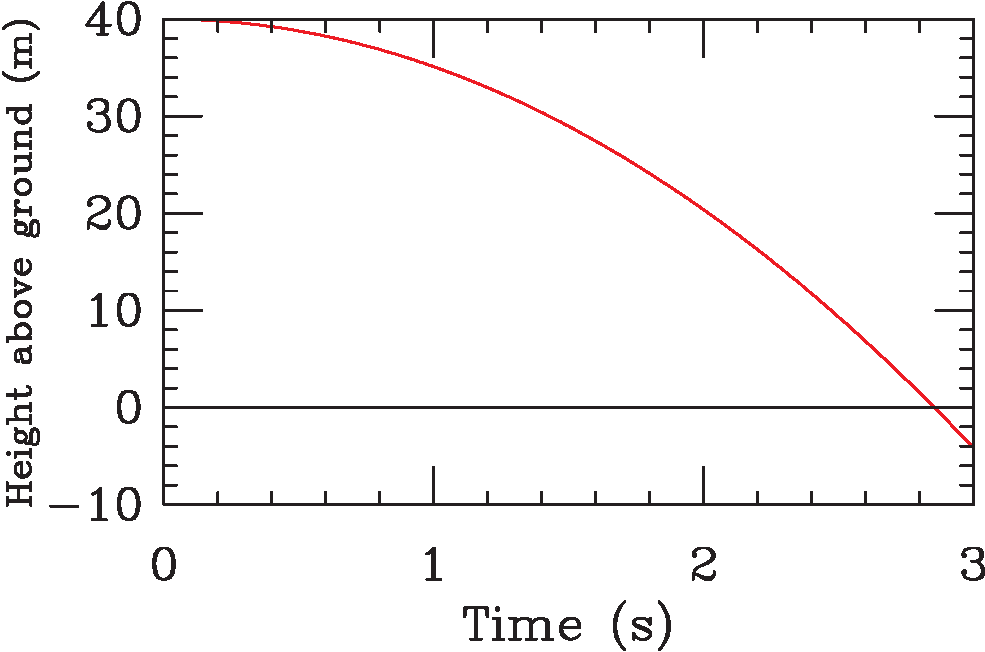
\includegraphics[width=0.7\textwidth]{falling-crop.pdf}}

\column{0.5\textwidth}
\color{Blue}
$$y(t) = (40 \,{\mathrm m}) - C t^2$$ \\
(C is some number; we'll learn what it is Thursday)

\end{columns}

\bigskip

\centerline{Both let us answer questions like ``When does the object hit the ground?''}

\bigskip

\begin{columns}
\column{0.5\textwidth}
\centerline {\color{Red}\large $\rightarrow$ ... the curve's x-intercept}
\column{0.5\textwidth}
\centerline{\color{Blue} \large $\rightarrow$ ... when $y(t)=0$}
\end{columns}

}

\frame{\frametitle{\textbf{Velocity: how fast position changes}}
\large
The slope of the position vs. time curve has a special significance. Here's one with a constant slope:

\medskip

\centerline{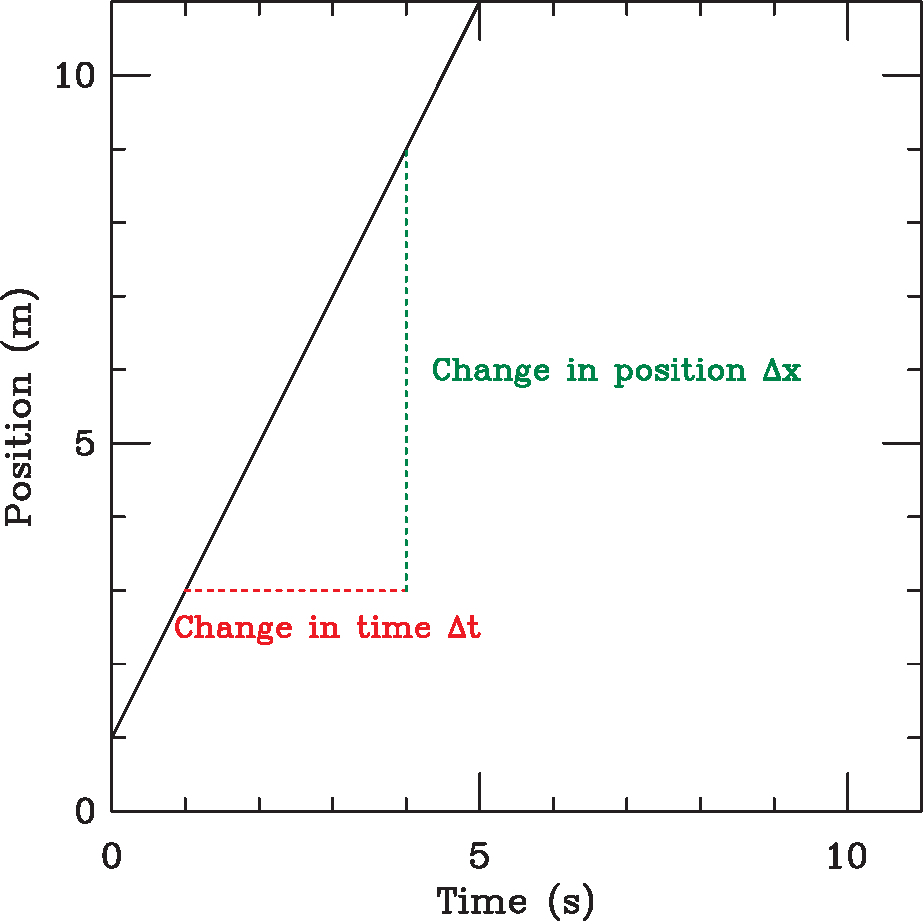
\includegraphics[width=0.4\textwidth]{constant-v-crop.pdf}}

\bigskip

\pause

Slope is $\frac{{\rm rise}}{{\rm run}}$ = $\frac{\Delta x}{\Delta t}$ = $\frac{2\,\rm m}{1 \, \rm s}$ = 2 meters per second (positive;
it could well be negative!)

\bigskip \pause

{\color{Red} $\rightarrow$ The slope here -- change in position over change in time -- is the {\bf velocity}!} Note that it can be
positive or negative, depending on which way the object moves.

}


\frame{\frametitle{\textbf{Constant-velocity motion: connecting graphs to algebra}}
\large
If an object moves with constant velocity, its position vs. time graph is a line:

\medskip

\centerline{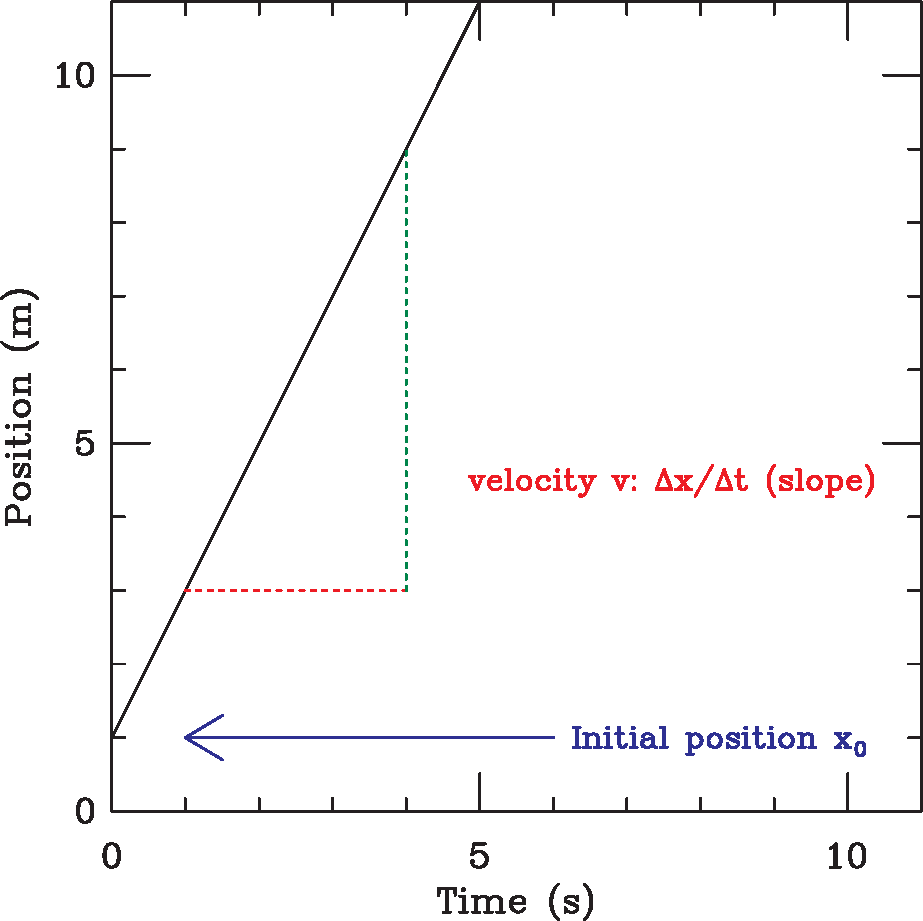
\includegraphics[width=0.4\textwidth]{constant-v-2-crop.pdf}}

We know the equation of a straight line is is $x = mt + b$ (using $t$ and $x$ as our axes).

\BI
\item{$m$ is the slope, which we identified as the velocity}
\item{$b$ is the vertical intercept, which we recognize as the value of $x$ when $t=0$}
\EI

We can thus change the variable names to be more descriptive:

\bigskip

\centerline{\Large{{\color{Red} $x(t) = vt + x_0$} (constant-velocity motion)}}

}

\frame{\frametitle{\textbf{Going from ``equations of motion'' to answers}}

\large

{\color{Red}$x(t) = vt + x_0$} is called an {\it equation of motion}; in this case, it is valid for constant-velocity motion.

\medskip

It gives you the same information as a position vs. time graph, but in algebraic form.

\bigskip
\bigskip

\normalsize

To solve real problems, we need to be able to translate physical questions into algebraic statements:
\bigskip
\bigskip

\BI
\item{``If a car starts at milepost 30 and drives at 50 mph, where is it an hour later?''}
\pause
\BI
\item{Using $x(t) = x_0 + vt$, with $x_0=30\, {\rm mi}$ and $v = 50 \frac{\rm mi}{\rm hr}$, calculate $x$ at $t=1\, {\rm hr}$}
\EI
\pause
\item{``When does a falling object hit the ground?''}
\pause
\BI
\item{If the ground is at $y=0$, then we ask: ``What is the value of $t$ when $y=0$?''}
\EI
\pause
\item{``When do two moving objects meet?''} 
\pause
\BI
\item{Write down $x_1(t)$ and $x_2(t)$, then ask ``At what time does $x_1 = x_2$?''}
\EI
\EI
}

\frame{\frametitle{\textbf{A rough problem-solving guide for constant-velocity motion}}

\large

A general framework for solving constant-velocity problems algebraically:

\begin{enumerate}
\item{Decide on a coordinate system: where is $x=0$, and which way is positive?}
\item{Write down the equation of motion $x(t)=x_0+vt$ for each object}
\item{Ask ``How can I translate the thing I'm looking for into an algebraic statement?''}
\item{Do the algebra!}
\end{enumerate}

\bigskip
\bigskip

}

\end{document}
